\chapter{PySide概述}

\section{PySide简介}
PySide6是Qt官方支持和维护的Python绑定库，它允许开发者在Python中创建基于Qt的图形用户界面（GUI）应用程序。与PyQt相比，PySide6在最新版本的Qt中得到了官方支持，并且使用LGPL许可证，这意味着你可以在自己的项目中使用PySide6，而不需要开源你的应用程序的源代码

简单来说，PySide6 就是将 Qt 6 提供的功能“翻译”成 Python 语言，让你可以用 Python 来开发图形界面应用程序。

\subsection{Qt 、PyQt 、PySide 之间的关系}
Qt 是一个广泛使用的框架，用于开发跨平台的图形用户界面（GUI）应用程序。它提供了创建桌面和移动应用程序的工具。

PyQt 和 PySide 是两种流行的 Python 绑定库，允许你用 Python 编写 Qt 应用程序。
\begin{enumerate}[label=\arabic*)]
    \item Qt：这是一个用 C++ 编写的核心框架，用于开发 GUI 应用程序。它包括小部件、图形、网络等库。
    \item PyQt：
    \begin{enumerate}[itemindent=1em,label=\arabic*)]
        \item 由 Riverbank Computing 开发。
        \item 提供了 Qt 库到 Python 的绑定。
        \item 通常使用 GPL 或商业许可证，这可能要求为专有软件购买许可证。
    \end{enumerate}
    
    \item PySide：
    \begin{enumerate}[itemindent=1em,label=\arabic*)]
        \item 由 Qt 公司（之前是诺基亚和 Digia）开发。
        \item 提供了 Qt 库到 Python 的绑定。
        \item 使用 LGPL 许可证，这允许更灵活的许可证，尤其适用于商业应用程序。
    \end{enumerate}
\end{enumerate}

PySide6/PyQt6都是基于Qt6, 它们之间的代码没什么区别；PySide2/PyQt5都是基于Qt5, 它们之间的代码也没什么区别。
以下代码可以相互替换
\begin{lstlisting}[style=demostyle,numbers=none]
from PySide6 import *
from PyQt6 import *
\end{lstlisting}
\begin{lstlisting}[style=demostyle,numbers=none]
from PySide2 import *
from PyQt5 import *
\end{lstlisting}

\subsection{PySide与PyQt的比较}
\begin{enumerate}[label=\arabic*)]
    \item 信号与槽的命名：

    下面代码等价：
    \begin{lstlisting}[style=demostyle,numbers=none]
    from PySide6.QtCore import Signal, Slot
    from PyQt6.QtCore import pyqtSignal as Signal, pyqtSlot as Slot
    \end{lstlisting}

    \item 枚举类型的快捷方式：
    \begin{lstlisting}[style=demostyle,numbers=none]
    Qt.Wednesday            # PySide6
    Qt.DayOfWeek.Wednesday  # PyQt6/PySide6
    \end{lstlisting}

    但是有\codeinline{qtpy}模块，使得PySide和PyQt可以通用，不需要修改代码,即使Python环境下只有 PyQt6 和 qtpy 模块，也可以运行 PySide6 的代码。
    \begin{lstlisting}[style=demostyle,numbers=none]
    from qtpy.QtCore import Qt
    \end{lstlisting}
\end{enumerate}



\subsection{主要模块}
\begin{enumerate}[label=\arabic*)]
    \item QtCore：
    提供核心功能，如事件处理、定时器、文件和目录操作、线程等。
    \item QtGui：
    提供图形功能，如 2D 图形绘制、字体、图像和窗口管理。
    \item QtWidgets：
    提供传统的桌面小部件，用于构建经典的用户界面组件。
    \item QtQuick 和 QML：
    支持现代的声明式用户界面设计，适用于创建动态和交互丰富的界面。
    \item QtNetwork：
    提供网络功能，如 TCP/IP 套接字、HTTP 请求等。
    \item QtSql：
    提供对 SQL 数据库的访问和操作功能。
\end{enumerate}


\section{安装PySide}
\url{https://doc.qt.io/qtforpython-6/quickstart.html#}
\begin{lstlisting}[style=demostyle,numbers=none]
$> conda create --name myenv python=3.9
$> conda activate myPySide
$> pip install pyside6
$> pip install pyside6==6.4.1

# 查看已安装的包
$> pip list | grep PySide6
$> pip show pyside6
Name: PySide6
Version: 6.7.2
Summary: Python bindings for the Qt cross-platform application and UI framework
Home-page: https://pyside.org
Author:
Author-email: Qt for Python Team <pyside@qt-project.org>
License: LGPL
Location: /home/tony/.application/Miniconda/envs/myPySide/lib/python3.9/site-packages
Requires: PySide6-Addons, PySide6-Essentials, shiboken6
Required-by:
\end{lstlisting}

\subsection{常见问题}

\begin{figure}[htpb]
    \centering
    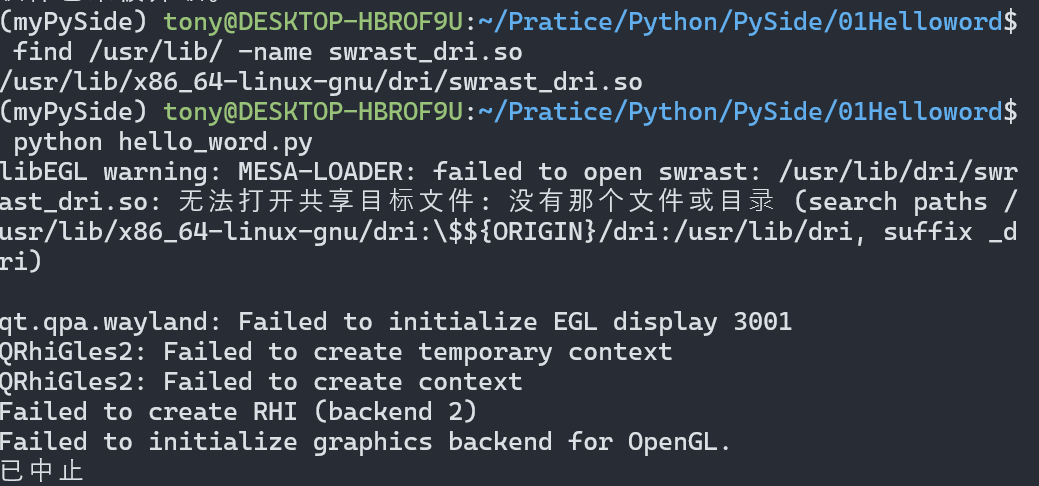
\includegraphics[width=0.6\textwidth]{part/图形化/pic/PySide/找不到swrast.png}
    \caption{找不到swrast}
    \label{fig:NotFoundSwrast}
\end{figure}

    
\subsubsection{PySide找不到libstdc++}
\begin{figure}[htpb]
    \centering
    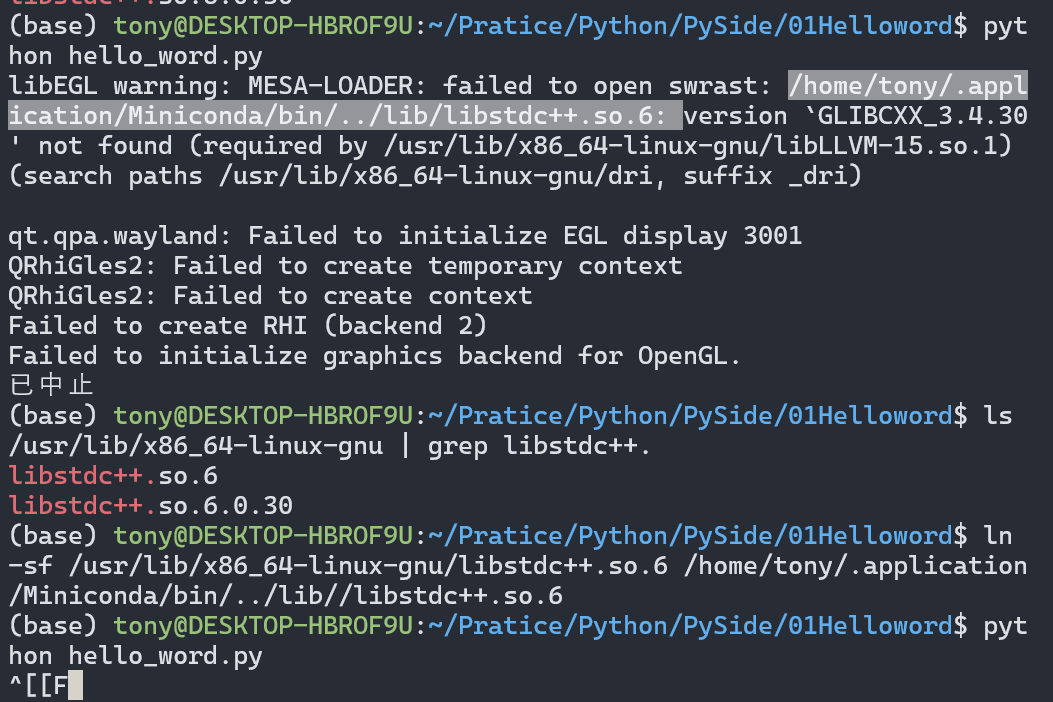
\includegraphics[width=0.6\textwidth]{part/图形化/pic/PySide/PySide找不到libstdc++.png}
    \caption{PySide找不到libstdc++}
    \label{fig:PySideNotFoundLibstdc++}
\end{figure}

\begin{lstlisting}[style=demostyle,numbers=none]
ln -sf /usr/lib/x86_64-linux-gnu/libstdc++.so.6 /home/tony/.application/Miniconda/bin/../lib/libstdc++.so.6
\end{lstlisting}

\subsubsection{conda的python版本与系统的版本不一致}

\begin{figure}[htpb]
    \centering
    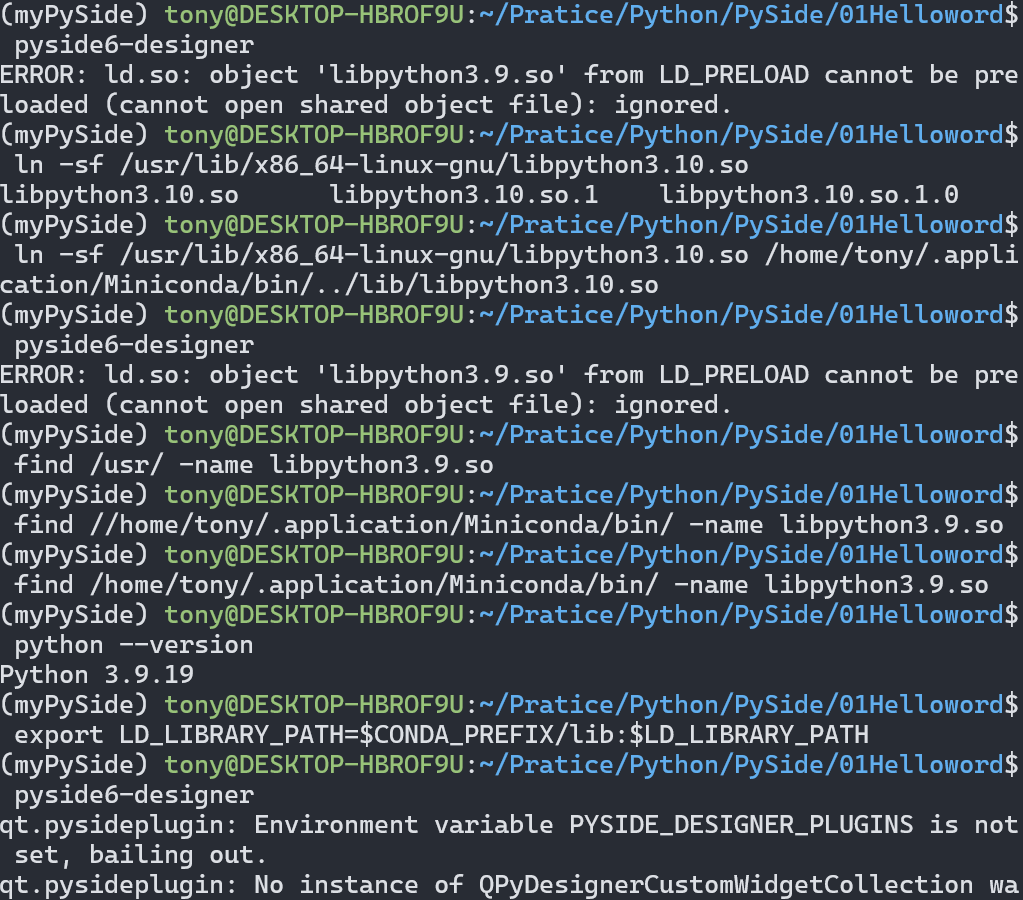
\includegraphics[width=0.6\textwidth]{part/图形化/pic/PySide/conda的python版本与系统的版本不一致.png}
    \caption{conda的python版本与系统的版本不一致}
    \label{fig:CondaPythonVersionNotMatch}
\end{figure}

\begin{lstlisting}[style=demostyle,numbers=none]
export LD_LIBRARY_PATH=$CONDA_PREFIX/lib:$LD_LIBRARY_PATH
\end{lstlisting}

